\def\PageLayout{single-no-print}
\def\DocLanguage{en}
\def\PackagesIncludeTikz{yes}
\def\PackagesIncludeBib{yes}

%%% Different page dimensions used on thesis
\def\PageLayoutSingle{single}
\def\PageLayoutSingleNoPrint{single-no-print}
\def\PageLayoutDouble{double}
\def\PageLayoutDoubleNoPrint{double-no-print}



%% Single page print
\ifx\PageLayout\PageLayoutSingle
\documentclass[a4paper,oneside,12pt]{report}
\setlength\textwidth{145mm}
\setlength\textheight{251mm}
\setlength\oddsidemargin{15mm}
\setlength\evensidemargin{15mm}
\setlength\topmargin{-0.4in}
\setlength\headsep{10mm}
\setlength\headheight{0mm}
\let\openright=\clearpage
\fi

%% Double page print
\ifx\PageLayout\PageLayoutDouble
% \documentclass[12pt,a4paper,twoside,openright]{report} % chapter will always start on the right side
\documentclass[12pt,a4paper,twoside]{report}
\setlength\textwidth{145mm}
\setlength\textheight{251mm}
\setlength\oddsidemargin{14.2mm}
\setlength\evensidemargin{0mm}
\setlength\topmargin{-0.4in}
\setlength\headsep{10mm}
\setlength\headheight{0mm}
\let\openright=\clearpage
% \let\openright=\cleardoublepage
\fi

%% Double page without space left for binding
\ifx\PageLayout\PageLayoutDoubleNoPrint
% \documentclass[12pt,a4paper,twoside,openright]{report} % chapter will always start on the right side
\documentclass[12pt,a4paper,twoside]{report}
\setlength\textwidth{145mm}
\setlength\textheight{251mm}
\setlength\oddsidemargin{9mm}
\setlength\evensidemargin{9mm}
\setlength\topmargin{-0.4in}
\setlength\headsep{10mm}
\setlength\headheight{0mm}
\let\openright=\clearpage
% \let\openright=\cleardoublepage
\fi

%% Single page without space left for binding
\ifx\PageLayout\PageLayoutSingleNoPrint
\documentclass[12pt,a4paper]{report}
\setlength\textwidth{145mm}
\setlength\textheight{251mm}
\setlength\oddsidemargin{9mm}
\setlength\evensidemargin{9mm}
\setlength\topmargin{-0.4in}
\setlength\headsep{10mm}
\setlength\headheight{0mm}
\let\openright=\clearpage

\fi




\def\LangCS{cs}
\def\LangEN{en}
\def\ConfirmExpr{yes}




%%% TiKz
% Memoize package needs to be loaded as soon as possible, in beamer even before document declaration
\ifx\PackagesIncludeTikz\ConfirmExpr
	\usepackage{memoize}
	\usepackage{collargs}
	\usepackage{tikz}
	\usepackage{tikz-cd}
	\usepackage{circuitikz}
	\mmzset{memo dir=memoize}
	\mmzset{auto={circuitikz}{memoize}}
	\mmzset{auto={tikzcdi}{memoize, verbatim}}
	\mmzset{auto={tikzpicture}{memoize, verbatim}}

	\usetikzlibrary{calc}
	\usetikzlibrary{fadings}
	\usetikzlibrary{shapes.geometric, arrows, positioning}

	\tikzstyle{layerheader} = [rectangle, minimum width=3cm, minimum height=1cm, text centered, draw=black, fill=gray!30]
	\tikzstyle{startstop} = [ellipse, minimum width=3cm, minimum height=1cm, text centered, draw=black, fill=red!30]
	\tikzstyle{process} = [rectangle, minimum width=3cm, minimum height=1cm, text centered, draw=black, fill=blue!20]
	\tikzstyle{decision} = [diamond, minimum width=2.5cm, minimum height=1cm, text centered, draw=black, fill=green!20]
	\tikzstyle{arrow} = [thick,->,>=stealth]
\fi




\ifx\DocLanguage\LangCS
	\usepackage[czech]{babel}
	\babelprovide[transforms = oneletter.nobreak]{czech} % non break on single letter words in czech
\else
	\usepackage[english]{babel}
\fi


\usepackage[T1]{fontenc}
\usepackage[utf8]{inputenc}
\usepackage{lmodern,textcomp}

\usepackage[a-2u]{pdfx}         % adding metadata to pdf with .xmpdata file
\usepackage{graphicx}						% inserting pictures
\usepackage{caption}						%	captions of figures
\usepackage{subcaption} 				% multiple figures in one figure environment
\usepackage{hyperref} 					% handling of hypertext
\usepackage{tabularx}           % table environment
\usepackage{xcolor,colortbl}    % more options for colors
\usepackage{textpos}            % more precise control over positioning of elements
\usepackage{longtable}          % longtable environment to enable multipage tables
\usepackage{fancyhdr}						% custom header and footer
\usepackage{xurl}								% extension to url handeling, allows linebreaks in urls and more special characters
\usepackage{enumitem}           % more options for labeling lists
\usepackage{multicol}           % simplest environment to achieve multiple columns

%%% Math packages
\usepackage{pgfplots}           % graphs
\usepackage{amsmath}						% extension for math
\usepackage{amsthm}							% environment for lemmas, proofs, theorems, etc.
\usepackage{amssymb} 						% math symbols
\usepackage{mathrsfs}  	        % math symbols
\usepackage{mathabx}						% math symbols
\usepackage{mathrsfs} 					% Fancy italic used to denote Hilbert spaces and such
\usepackage{bbm} 							  % blackboard variants of computer Modern fonts useful for number groups, mean value notation
\usepackage{esint} 						  % adds more integrals
\usepackage{accents} 						% multiple mathematical accents
\usepackage{arcs} 							% arcs over and under words
\usepackage{steinmetz} 					% Steinmetz notation for complex numbers
\usepackage{mathtools}


%%% Basic configuration of packages
\def\columnseprulecolor{\color{black}}
\setlength{\columnseprule}{0.3pt}

\hypersetup{pdfborder=0 0 0}
\hypersetup{unicode}
\hypersetup{breaklinks=true}

\pgfplotsset{compat=1.15}

%%% Bibliography
\ifx\PackagesIncludeBib\ConfirmExpr
	\usepackage[backend=biber,style=iso-numeric,sortlocale=cs_CZ, url=true]{biblatex}

	\DeclareFieldFormat{labelnumberwidth}{\mkbibbrackets{#1}} % force biblatex to make brackets around numbers
	\ExecuteBibliographyOptions{maxcitenames=2} % In citation with full bibliography entry cite just two names at max, per ISO 690

	\let\familynameformat=\textsc % Use caps-and-small-caps for family names in ISO 690 style.

	% We want to separate multiple authors in citations by commas
	% (while we use semicolons in the bibliography as per the ISO standard)
	\DeclareDelimFormat[textcite]{multinamedelim}{\addcomma\space}
	\DeclareDelimFormat[textcite]{finalnamedelim}{\space and~}
\fi



%%% Minted
\ifx\PackagesIncludeMinted\ConfirmExpr
	\usepackage{minted}
	\setminted{mathescape,escapeinside=@@,linenos,numbersep=5pt,frame=lines,breaklines,tabsize=2,framesep=2mm}
\fi

%%% Please fill in basic information on your thesis, which will be automatically
%%% inserted at the right places. You need to replace \xxx{...} by real data.

% Type of your thesis:
%	"bc" for Bachelor's
%	"mgr" for Master's
%	"phd" for PhD
%	"rig" for rigorosum
% "sem" for semestral
\def\ThesisType{bc}

\def\DocLanguage{en}


\def\ThesisTitle{\xxx{Thesis title}}

\def\ThesisTitleShort{\xxx{Surveillance FMCW radar}}

\def\ThesisAuthor{\xxx{Havránek Kryštof}}

\def\MontSubmitted{\xxx{MONTH}}

\def\YearSubmitted{\xxx{YEAR}}

\def\Institution{Czech Technical University in Prague}

\def\Faculty{\xxx{Name of the department}}

\def\Department{\xxx{Faculty of Electrical Engineering}}

\def\Supervisor{\xxx{Ing. Viktor Adler, Ph.D}}

\def\SupervisorsDepartment{\xxx{department}}

\def\StudyProgramme{\xxx{Elektronika a komunikace}}

\def\Dedication{%
\xxx{Dedication.}
}

\def\Abstract{%
\xxx{Use the most precise, shortest sentences that state what problem the
thesis addresses, how it is approached, pinpoint the exact result achieved, and
describe the applications and significance of the results. Highlight anything
novel that was discovered or improved by the thesis. Maximum length is 200
words, but try to fit into 120. Abstracts are often used for deciding if
a reviewer will be suitable for the thesis; a well-written abstract thus
increases the probability of getting a reviewer who will like the thesis.}
}

% 3 to 5 keywords (recommended) separated by \sep
% Keywords are useful for indexing and searching for the theses by topic.
\def\ThesisKeywords{%
\xxx{keyword\sep key phrase}
}

% If any of your metadata strings contains TeX macros, you need to provide
% a plain-text version for use in XMP metadata embedded in the output PDF file.
% If you are not sure, check the generated thesis.xmpdata file.
\def\ThesisAuthorXMP{\ThesisAuthor}
\def\ThesisTitleXMP{\ThesisTitle}
\def\ThesisKeywordsXMP{\ThesisKeywords}
\def\AbstractXMP{\Abstract}

% If your abstracts are long and do not fit in the infopage, you can make the
% fonts a bit smaller by this setting. (Also, you should try to compress your abstract more.)
\def\InfoPageFont{}
%\def\InfoPageFont{\small}  % uncomment to decrease font size

% If you are studing in a Czech programme, you also need to provide metadata in Czech:
% (in English programmes, this is not used anywhere)

\def\ThesisTitleCS{\xxx{Název práce česky}}
\def\DepartmentCS{\xxx{Název katedry česky}}
\def\DeptTypeCS{\xxx{Katedra}}
\def\SupervisorsDepartmentCS{\xxx{katedra vedoucího}}
\def\StudyProgrammeCS{\xxx{studijní program}}

\def\ThesisKeywordsCS{%
\xxx{klíčová slova\sep klíčové fráze}
}

\def\AbstractCS{%
\xxx{Abstrakt práce přeložte také do češtiny.}
}


%%% This file contains definitions of various useful macros and environments %%%
%%% Please add more macros here instead of cluttering other files with them. %%%

\def\LangCS{cs}
\def\LangEN{en}


%%% Minor tweaks of style

% These macros employ a little dirty trick to convince LaTeX to typeset
% chapter headings sanely, without lots of empty space above them.
% Feel free to ignore.
\makeatletter
\def\@makechapterhead#1{
  {\parindent \z@ \raggedright \normalfont
   \Huge\bfseries \thechapter. #1
   \par\nobreak
   \vskip 20\p@
}}
\def\@makeschapterhead#1{
  {\parindent \z@ \raggedright \normalfont
   \Huge\bfseries #1
   \par\nobreak
   \vskip 20\p@
}}
\makeatother

% make chaptermark non uppercase
\renewcommand{\chaptermark}[1]{%
  \markboth{#1}{}}

% This macro defines a chapter, which is not numbered, but is included in the table of contents.
\def\chapwithtoc#1{
\chapter*{#1}
\addcontentsline{toc}{chapter}{#1}
}

% Slightly less strict rules for placing breaklines inside words
\lefthyphenmin=2
\righthyphenmin=2

% Draw black "slugs" whenever a line overflows, so that we can spot it easily.
% \overfullrule=1mm

% Empty page

\ifx\DocLanguage\LangEN
\newcommand\blankpage{
\newpage
\begin{center}
\vspace*{\fill}
  {Empty page}
\vspace*{\fill}
\end{center}
}

\else
\newcommand\blankpage{
\newpage
\begin{center}
\vspace*{\fill}
  {Prázdná strana}
\vspace*{\fill}
\end{center}
}
\fi


%%% Macros for definitions, theorems, claims, examples, ... (requires amsthm package)
\makeatletter
\def\th@plain{%
  \thm@notefont{}% same as heading font
  \itshape % body font
}
\def\th@definition{%
  \thm@notefont{}% same as heading font
  \normalfont % body font
}
\makeatother

\ifx\DocLanguage\LangEN
\theoremstyle{plain}
\newtheorem{thm}{Theorem}
\newtheorem{lemma}[thm]{Lemma}
\newtheorem{claim}[thm]{Claim}
\newtheorem{defn}{Definition}

\theoremstyle{remark}
\newtheorem*{cor}{Corollary}
\newtheorem*{rem}{Remark}
\newtheorem*{example}{Example}

\else
\theoremstyle{plain}
\newtheorem{thm}{Teorém}
\newtheorem{lemma}[thm]{Lemma}
\newtheorem{claim}[thm]{Tvrzení}
\newtheorem{defn}{Definice}

\theoremstyle{remark}
\newtheorem*{cor}{Důsledek}
\newtheorem*{rem}{Připomínka}
\newtheorem*{example}{Například}

\fi


%%% Tweaks for tables
\newcommand{\pulrad}[1]{\raisebox{1.5ex}[0pt]{#1}}
\newcommand{\mc}[1]{\multicolumn{1}{c}{#1}}
\newcolumntype{C}[1]{>{\centering\arraybackslash}p{#1}}

%%% TODO items
\newcommand{\xxx}[1]{\textcolor{red!}{#1}}


%%% Groups of different numbers, average value
\DeclareMathOperator{\R}{\mathbb{R}}
\DeclareMathOperator{\N}{\mathbb{N}}
\DeclareMathOperator{\Q}{\mathbb{Q}}
\DeclareMathOperator{\C}{\mathbb{C}}
\DeclareMathOperator{\F}{\mathbb{F}}
\DeclareMathOperator{\Z}{\mathbb{Z}}

\DeclareMathOperator{\coord}{\text{coord}}
\DeclareMathOperator{\mgrad}{\text{grad}\,}
\DeclareMathOperator{\mdiv}{\mathrm{div}\,}
\DeclareMathOperator{\mrot}{\mathrm{rot}\,}

%%% Comments inside of mathematical equations, useful for simple substitutions and such
\newcommand{\lcom}{\left\langle\left\langle} %% deprecated
\newcommand{\rcom}{\right\rangle\right\rangle} %% deprecated
\newcommand{\com}[1]{\left\langle\left\langle #1 \right\rangle\right\rangle}

%%% Equals with text over it
\DeclareMathOperator{\eqlh}{\mathrel{\stackrel{\makebox[0pt]{\mbox{\normalfont\tiny L'H}}}{=}}}
\DeclareMathOperator{\eqpp}{\mathrel{\stackrel{\makebox[0pt]{\mbox{\normalfont\tiny PP}}}{=}}}
\newcommand{\eqi}[1]{\mathrel{\stackrel{\makebox[0pt]{\mbox{\normalfont\tiny $#1$}}}{=}}}
\newcommand{\rai}[1]{\mathrel{\stackrel{\makebox[0pt]{\mbox{\normalfont\tiny $#1$}}}{\rightarrow}}}

%% Different lines under text
\newcommand*{\ucheck}[1]{\underaccent{\check}{#1}}
\newcommand*{\uwidecheck}[1]{\underaccent{\widecheck{\hphantom{#1}}}{#1}}
\def\doubleunderline#1{\underline{\underline{#1}}}\makeatletter

%%% Handle " in tikzcd
\newenvironment{tikzcdi}{\shorthandoff{"}\begin{tikzcd}}{\end{tikzcd}\shorthandon{"}}%

%%% Macros for statistics and probability theory
\DeclareMathOperator{\pr}{\textsf{P}}
\DeclareMathOperator{\E}{\textsf{E}\,}
\DeclareMathOperator{\var}{\textrm{var}}
\DeclareMathOperator{\sd}{\textrm{sd}}
\DeclareMathOperator{\ED}{\mathbb{E}}

%%% Other math tweaks
\newcommand{\goto}{\rightarrow}
\newcommand{\gotop}{\stackrel{P}{\longrightarrow}}
\newcommand{\maon}[1]{o(n^{#1})}
\newcommand{\abs}[1]{\left|{#1}\right|}
\ExplSyntaxOn
\NewDocumentCommand{\intd}{m}
{
    \int \clist_map_inline:nn { #1 } { \mathrm{d} ##1 \, }
}
\ExplSyntaxOff % expands \intd{x,y} into \int \mathrm{d}x \mathrm{d}y, used primarily in quantum physics
\newcommand{\isqr}[1]{\frac{1}{\sqrt{#1}}}
\newcommand{\T}[1]{#1^\top}

%% braket notation
\DeclarePairedDelimiter\bra{\langle}{\rvert}
\DeclarePairedDelimiter\ket{\lvert}{\rangle}
\DeclarePairedDelimiterX\braket[2]{\langle}{\rangle}{#1\,\delimsize\vert\,\mathopen{}#2}

%%% Environment with different font size
\newenvironment{localsize}[1]
{%
  \clearpage
  \let\orignewcommand\newcommand
  \let\newcommand\renewcommand
  \makeatletter
  \input{bk#1.clo}%
  \makeatother
  \let\newcommand\orignewcommand
}
{%
  \clearpage
}

%%% Prostředí pro tabulky s centrováním textu v buňce
\newcolumntype{C}[1]{>{\centering\arraybackslash}p{#1}}


% Generate XMP metadata file (*.xmpdata)
% one needs to set AuthorXMP, TitleXMP, KeywordsXMP, AbstractXMP

{
\catcode`\%=12
\global\edef\percenthack{%}
}

{
\def\xxx#1{#1}
\def\sep{\string\sep\space}
\let~=\space

\newwrite\xmp
\immediate\openout\xmp=\jobname.xmpdata
\immediate\write\xmp{\percenthack\space Generated automatically from metadata.tex}
\def\xmpitem#1#2{\immediate\write\xmp{\string#1{#2}}}
\xmpitem\Author\AuthorXMP
\xmpitem\Title\TitleXMP
\xmpitem\Keywords\KeywordsXMP
\xmpitem\Subject\AbstractXMP
\xmpitem\Publisher{Czech Technical University in Prague}
\immediate\closeout\xmp
}


\def\PageLayoutSingle{single}
\def\PageLayoutSingleNoPrint{single-no-print}
\def\PageLayoutDouble{double}
\def\PageLayoutDoubleNoPrint{double-no-print}

% Overwrite default chapter behaviour to control what style is used
\makeatletter
    \let\stdchapter\chapter
    \renewcommand*\chapter{%
    \@ifstar{\starchapter}{\@dblarg\nostarchapter}}
    \newcommand*\starchapter[1]{%
        \stdchapter*{#1}
        \thispagestyle{plain}
        \markboth{\MakeUppercase{#1}}{}
    }
    \def\nostarchapter[#1]#2{%
        \stdchapter[{#1}]{#2}
        \thispagestyle{fancy}
    }
\makeatother




%%% Style for TOC, introduction, conclusion, bibliography and such
\fancypagestyle{plain}{
  \fancyhf{}
  \renewcommand{\headrulewidth}{0.4pt}
  \renewcommand{\footrulewidth}{0.4pt}
  \fancyhead[C]{}
  \fancyhead[L]{}
  \fancyfoot[L]{\Institution}
  \fancyfoot[C]{}
  \fancyfoot[R]{\thepage}
}

\ifx\PageLayout\PageLayoutDouble
\fancypagestyle{fancy}{%
  \fancyhf{}%
  \renewcommand{\headrulewidth}{0.4pt}%
  \renewcommand{\footrulewidth}{0.4pt}%
  \fancyhead[C]{}
	\fancyhead[LE]{\textbf{\thechapter. \leftmark}}
	\fancyhead[RO]{\textbf{\rightmark}}
  \fancyfoot[L]{\Institution}
  \fancyfoot[C]{}
  \fancyfoot[R]{\thepage}
}
\fi

\ifx\PageLayout\PageLayoutDoubleNoPrint
\fancypagestyle{fancy}{%
  \fancyhf{}%
  \renewcommand{\headrulewidth}{0.4pt}%
  \renewcommand{\footrulewidth}{0.4pt}%
  \fancyhead[C]{}
	\fancyhead[LE]{\textbf{\thechapter. \leftmark}}
	\fancyhead[RO]{\textbf{\rightmark}}
  \fancyfoot[L]{\Institution}
  \fancyfoot[C]{}
  \fancyfoot[R]{\thepage}
}
\fi


\ifx\PageLayout\PageLayoutSingle
\fancypagestyle{fancy}{%
  \fancyhf{}%
  \renewcommand{\headrulewidth}{0.4pt}%
  \renewcommand{\footrulewidth}{0.4pt}%
  \fancyhead[C]{}
	\fancyhead[L]{\textbf{\thechapter. \leftmark}}
  \fancyfoot[L]{\Institution}
  \fancyfoot[C]{}
  \fancyfoot[R]{\thepage}
}

\fi

\ifx\PageLayout\PageLayoutSingleNoPrint
\fancypagestyle{fancy}{%
  \fancyhf{}%
  \renewcommand{\headrulewidth}{0.4pt}%
  \renewcommand{\footrulewidth}{0.4pt}%
  \fancyhead[C]{}
	\fancyhead[L]{\textbf{\thechapter. \leftmark}}
  \fancyfoot[L]{\Institution}
  \fancyfoot[C]{}
  \fancyfoot[R]{\thepage}
	}

\fi


\addbibresource{bibliography.bib}

\newcommand{\sidar}{SiRad Easy\textsuperscript{\copyright}}
\newcommand{\boldred}[1]{\textbf{\textcolor{red}{#1}}}
\newcommand{\boldblue}[1]{\textbf{\textcolor{blue}{#1}}}
% \newcommand{\red}[1]{\textcolor{red}{#1}}


\begin{document}

\include{doc_paper_title_page_en}

\tableofcontents

\newpage
\pagenumbering{arabic}
\setcounter{page}{1}


\chapter*{Introduction}
\addcontentsline{toc}{chapter}{Introduction}

While two-axis rotary platforms are fairly common in the world of machining, they are often prohibitively expensive, and their operational parameters are frequently unnecessarily precise \cite{carl}.
As for an application as radar platform where the angular width of the main lobe can span several degrees \cite{sidarMAN} high precision is not required.
Additionally, most driving boards, typically in the form of G-code/M-code interpreters, are not designed to provide frequent uplink about their current position \cite{duet}.
Feature that is crucial in order to be able to counteract the movement of the platform in post processing.

This thesis focuses on designing and building a cost-effective two-axis rotary platform with parameters purposefully chosen to match the requirements of a radar system.
This necessitates achieving timely and deterministic movement of the stepper motors, allowing radar data processing to accurately account for platform motion during post-processing.
In addition the platform needs to be as easy to operate for an end user as possible.
Allowing easy integration into projects.

To achieve this, a three-layer command processing architecture is proposed and implemented.
This architecture enables almost seamless transitions between commands.
Additionally, this approach allows for preprogramming entire movement sequences that can be executed continuously without any user intervention.

The first chapter  outlines the basic design requirements for the platform based on radar parameters.
The following chapter focuses on the hardware aspects of the project, including the electronic components and mechanical design.
The final chapter is dedicated to the software that controls the platform.

\pagestyle{fancy}

\chapter{FMCW Radar Fundamentals}

\boldred{TODO: Consider some semi-introductory chapter before this one. Also the name "Basics of FMCW Radar" is not very good.}

As opposed to classical continuos wave (CW) radars Frequency Modulated Continuous Wave (FMCW) radars broadcast a signal not on a single frequency but with linear sweep across a range of frequencies.
Such approach allows computing a range estimation without requiring a pulsing signal.
This is while the capability to measure speed of the target using doppler shift is still maintained.
However the calculation of speed more complex than in case of broadcast on a single frequency.

The MW suffix in FMCW radar is used to denote that the radar operates in microwave range of frequencies.
Such frequencies enable the antenna array to be small, enabling even on chip internaration.
Also MM part of radio spectrum is generally license free \cite{spektrumCTU} and offers large bandwiths -- limiting possible interference.

\section{Comparison FMCW Radar to Pulse Radar}

Distance measurement with radar predates an invent of FMCW radar by a few decades.
Traditional approaches relied predominantly on sending pulsing the signal electromagnetic radiation and measuring time it takes for the signal to return.
On such radars speed can be calculated traditionally using Doppler effect as
\begin{equation}
	v = \frac{f_\mathrm{dop} c_o}{2f_\mathrm{rad}},
	\label{eq:dopler}
\end{equation}
where $f_\mathrm{dop}$ is doppler frequency, $c_o$ is speed of light and $f_\mathrm{rad}$ is frequency of the radar signal.
And distance was tied to time of flight $t$ of the signal as
\begin{equation}
	d = \frac{c_o \cdot t}{2}.
	\label{eq:distance}
\end{equation}

Such approach is on paper simpler and more intuitive however it has several drawbacks that seriously limit its precision and usability especially in close range applications.
In order to achieve a good resolution in distance measurement the pulse must be very short.
However in order to to impede on radars capabilities (need to maintain strong signal-to-noise ration SNR over long distances) the power of the pulses must stay the same even when the duty cycle is dramatically increased \cite{jankiraman2018}.

Transmitting with high average power is problematic legally and technically.
It can result in interfering with other devices not to mention circuity to drive high power radars is bulky and expensive often requiring use of high voltages and vacuum tubes.
Thus pulsed radars are predominantly used in application where high resolution in range is not needed such as long range detection.

One major advantage of pulsed radar is the ease of processing data.
On FMCW radar the there is a entanglement of distance and speed readings as there is both frequency change due to Doppler effect and the frequency sweep itself.

\section{Basic principles of ideal FMCW radar}

Let us picture an ideal FMCW radar system sending a chirp with frequency frequency sweep from $f_\mathrm{c}$ to $f_\mathrm{c}+BW$ and receiving the exact same signal signal after it has been reflected from a static target.

\begin{figure}[h!]
	\centering
\begin{tikzpicture}[>=latex, scale=1]

% Axes
\draw[->] (0, 0) -- (8, 0) node[below] {$t$};
\draw[->] (0, 0) -- (0, 5) node[left] {$f$};

% Horizontal lines for BW
\draw[dashed] (0, 4.5) -- (7.5, 4.5);
\draw[dashed] (0, 1) -- (7.5, 1);
\draw[dashed] (2.5, -0.05) -- (2.5, 4.7);

% Labels for fc and BW
\node[left] at (0, 1) {$f_c$};
\draw[<->] (-0.5, 1) -- (-0.5, 4.5) node[midway,left] {$BW$};

% Triangular wave for Tx
\draw[thick,blue] (0, 1) -- (2.5, 4.5);
\draw[thick,blue]	(2.5, 1) -- (5, 4.5);
\draw[thick, dashed, blue] (5, 1) -- (6, 2.4);

% Triangular wave for Rx (offset version)
\draw[thick,red] (0.5, 1) -- (3, 4.5);
\draw[thick,red] (3, 1) -- (5.5, 4.5);
\draw[thick, dashed, red] (5.4, 1) -- (6.4, 2.4);

% Label for Tch
	\draw[-] (2.5, -0.05) -- (2.5, 0.05) node[below] {$T_{\text{ch}}$};

% Labels for Tx and Rx
\node[blue] at (4.2, 4.1) {\small Tx};
\node[red] at (5.3, 3.7) {\small Rx};

% Sweep slope and fb
\draw[<->] (1, 1) arc[start angle=0, end angle=55, radius=1];
\node at (1.5, 1.3) {\small $k_{\text{sw}}$};
\draw[<->] (1.5, 2.37) -- (1.5, 3.12) node[above, left] {$f_b$};

% Small time delay (tau)
\draw[<->] (2.5, 0.7) -- (3, 0.7) node[midway,below] {$\tau$};

\end{tikzpicture}

	\caption[]{Ideal relation of frequency and time for received and sent signal}
	\label{fig:fmcw_ideal}
\end{figure}

We can clearly see that in given time $t$ the frequency spread from sent signal to received signal is proportional to the time delay $\tau$.
However doing some simple subtraction in spectrogram of the both signals isn't really feasible -- the calculation need to take a smarter approach.


Let us define the chirp slope $k_\mathrm{sw}$ we can describe the change in frequency of the received signal as
\begin{equation}
	\Delta f_\mathrm{s}(t) = k_\mathrm{sw}t = \frac{BW}{T_\mathrm{ch}} t,
	\label{eq:deltaf}
\end{equation}
where $t$ is the time goes from 0 to chirp length $T_\mathrm{ch}$. Standard equation of FM signal can be written as
\begin{equation}
	s_\mathrm{t}(t) = A \cos\left(\omega_c t + 2\pi \int_{0}^{t} f_\mathrm{s}(t) \mathrm{d}t\right),
	\label{eq:fm}
\end{equation}
where $A$ is amplitude of the signal, $\omega_c$ is carrier frequency and $f(s)$ is frequency of the signal. Substituting \ref{eq:deltaf} into \ref{eq:fm} we get the signal borrowed from the radar
\begin{equation}
	s_\mathrm{t}(t) = A \cos(\omega_c t + \pi k_\mathrm{sw}t^2).
	\label{eq:fm2}
\end{equation}

Signal bounced back from the target will have the same equation with the only difference being the time delay $\tau$,
\begin{equation}
	s_\mathrm{r}(t) = A \cos(\omega_c (t - \tau) + \pi k_\mathrm{sw}(t - \tau)^2).
	\label{eq:fm3}
\end{equation}
Now we can calculate the product of the two signals, this can be done easily in the real world using a frequency mixer. This is done with the standard formula $\cos(\alpha)\cos\beta = \frac{1}{2}(\cos(\alpha-\beta)+\cos(\alpha+\beta))$
The result of the multiplication is
\begin{align}
	s(t) = s_\mathrm{r}(t) \cdot  s_\mathrm{t}(t) &= \frac{A^2}{2}\cos\left(2(\omega_c - 2\pi k_\mathrm{sw}T_\tau)t + 2\pi k_{sw}t^2 + (\pi k_\mathrm{sw} \tau^2 - \omega_c \tau) \right)+ \nonumber \\
	&+\frac{A^2}{2} \cos\left(2\pi k_\mathrm{sw} \tau t + (\omega_c \tau - \pi k_\mathrm{sw} \tau^2)\right).
	\label{eq:fm4}
\end{align}
First additive term will lead to a signal with very high frequency, well above $2\omega_c$, this term doesn't carry any useful information and is usually filtered out -- either by low pass filter or the frequency mixer itself \cite{graham2015}.
Second term is so call beat signal whole frequency is directly proportional to the time delay $\tau$.
Applying a first time derivative to the cosine argument we get the frequency of the beat signal.
\begin{equation}
	f_\mathrm{b} = \frac{1}{2\pi}\frac{\partial}{\partial t} \left(2\pi k_\mathrm{sw} \tau t + (\omega_c \tau - \pi k_\mathrm{sw} \tau^2)\right) = k_\mathrm{sw} \tau.
	\label{eq:fb}
\end{equation}

Calculating the distance to the target is now trivial, delay $\tau$ is equal to the time it takes for the signal to travel to the target and back
\begin{equation}
	R = \frac{c_0 \tau}{2},
	\label{eq:distance2}
\end{equation}
Substituting \ref{eq:fb} into \ref{eq:distance2} we get equation for distance
\begin{equation}
	R = \frac{c_0 f_\mathrm{b}}{2k_\mathrm{sw}}= \frac{c_o f_\mathrm{b} T_{\mathrm{ch}}}{2 BW}.
	\label{eq:distance3}
\end{equation}


\subsection{Limits of Range Measurement}

Absolute limit for maximal distance is given by the time it takes for the signal to travel from the radar to the target and back.
Would the distance be greater than a time of single chirp the signal would be interpreted as coming from a closer target.
That gives us an maximal limit on beat frequency $f_\mathrm{b} = BW$.

However in most case the limit will imposed not by $T_\mathrm{ch}$ respectively $BW$ but by our sampling frequency $f_\mathrm{s}$.
In order to avoid aliasing the Nyquist-Shannon theorem must be satisfied thus limiting the maximal beat frequency to $f_\mathrm{s}/2$ and giving us maximal distance of
\begin{equation}
	R = \frac{c_o f_\mathrm{s}}{4k_\mathrm{sw}}.
	\label{eq:distance4max}
\end{equation}

While sampling with frequency $f_\mathrm{s}$ we get $N =\mathrm{f}_\mathrm{s} T_\mathrm{ch}$ samples. Applying a Discrete Fourier Transform (DFT) to the signal we get $N$ samples in spectrum with frequency resolution of
\begin{equation}
	\upDelta f_\mathrm{b} = \frac{f_\mathrm{s}}{N} = \frac{1}{T_{ch}},
	\label{eq:resolution}
\end{equation}
we can see that the resolution of spectrum is inversely proportional to the chirp length, however it doesn't depend on sampling frequency \cite{jankiraman2018}.
Now we can enter $\upDelta f_\mathrm{b}$ into \ref{eq:distance3} to get the minimal distance that can be measured as
\begin{equation}
	\upDelta R = \frac{c_o}{2BW}
	\label{eq:distance5min}
\end{equation}
Thus in order to increase resolution in range a wider bandwidth is needed.





\subsection{Speed Measurement}

In order to demonstrate the effect of moving target on the beat frequency we can redefine the time delay $\tau$ as
\begin{equation}
	\tau = \frac{2(R_0+vt)}{c_o}
	\label{eq:tau}
\end{equation}
where $R_0$ is the initial distance to the target and $v$ is the radial speed of the target.
Within a single chirp there is no way to distinguish between the effects distance and speed of the target -- thus multiple chirps are needed.
Rewriting \label{eq:tau} as
\begin{equation}
	\tau = \frac{2(R_0 v(nT_\mathrm{ch} + t_\mathrm{s}))}{c_0}
	\label{eq:tau2}
\end{equation}
where $n$ is the number of chirps, $T_\mathrm{ch}$ is the chirp length and $t_\mathrm{s}$ denotes time withing  a single chirp ($0 \leq t_\mathrm{s} \leq T_\mathrm{ch}$).
Substituting \ref{eq:tau2} into low frequency part \ref{eq:fm4} leads to very complex equation, however according to \cite{graham2015} most of the terms can be neglected leading us to
\begin{equation}
	s(t_\mathrm{s}, n) = \frac{A^2}{2} \cos\left(\frac{4\pi k_\mathrm{sw} R_0}{c_0} t_\mathrm{s} + \frac{2\omega_c v n}{c_0} T_\mathrm{ch} + \varphi_0 \right),
	\label{eq:fb2}
\end{equation}
where $\varphi_0$ is a phase shift given by the initial distance to the target.
Its clear that first element describes predominantly the distance to the target and the second one the speed of the target.
We can also see that speed will not affect a beat frequency in a single spectrum but will lead to a phase shift across multiple spectrums.

% 2D FFT
% speed resolution





\section{AoA Estimation of FMCW Radar}

\chapter{\sidar}

\boldred{TODO: Consider whether to have it as a chapter or just section under chapter dealing with FMCW technology itself.}

\section{24 GHz Header Simulation}




\chapter{Rotary Platform}

Following chapter outlines design process and operation of a rotary platform specifically designed for \sidar radar system.

\section{Platform Design Parameters}


To begin, it is essential to outline the fundamental requirements for the platform.
These stem from the physical capabilities of the radar system, SiRad Easy evalutions kit, and requirements for the software.

\subsection{Physical Capabilities}

\boldred{TODO: Should be more tied to the radar system - especially in regard to the radiation pattern of 24 GHz header.}

The primary constraints on the physical design arise from the radar's radiation pattern (Both 24 and 122 GHz headers are accounted for.), as it is crucial to minimize strong reflections from the platform's structure. According to the 122 GHz transceiver datasheet, the angular width at -3 dB is approximately $\pm30\text{°}$ in both the E-plane and H-plane \cite{sidarTRX}. With the addition of a radar dome the value decreases to $\pm4\text{°}$ \cite{sidarMAN}.

The radiation pattern for the 24 GHz microstrip patch antenna is not explicitly provided by the manufacturer. However, based on similar designs, a conservative estimate of $\pm15\text{°}$ is adopted, informed by \cite{patch1} and \cite{patch2}. Considering these values, we set a reasonably forgiving clearance limit of $\pm45\text{°}$ in front of the radar.

One can also see that significant cost cutting can be done in the area of precision of the platform.
As the radar system has relatively low angular resolution the sub degree control of commercial solutions is not needed.
This allows basic 200 steps NEMA17 stepper motors be used with optional microstepping to increase smoothness of movement.


In terms of speed, due to the radar system's relatively low polling rate (1 Mbit/s \cite{sidarMAN}), high-speed movement is unnecessary. The manufacturer specifies a maximum update frequency of 50 Hz, equating to a new update every 20 ms \cite{sidarMAN}.
Using the following equation:
%
\begin{equation}
  t_{\mathrm{angle}} = \frac{60}{360\cdot N_{\mathrm{RMP}}} \cdot  \alpha,
  \label{eq:poll}
\end{equation}
%
where $t_{\mathrm{angle}}$ is time between spend on traveling angle of $\alpha $ in seconds and $N_{\mathrm{RMP}}$ is number of rotations per minute, we can calculate that even for low RPM of 60 an angle of 8 degrees the platform travels (angular width of main lobe for 122 GHz radar) in 10 ms.

\subsection{Software Requirements}

Given its widespread adoption as an industry standard for controlling multi-axis machines, G-code over serial is a natural choice for the platform's communication format. Beyond the basic functionality typically offered by G-code interpreters, the platform must support additional features to reduce the user's manual control burden. These features include the ability to define movement limits and preprogram sequences of movements for autonomous execution by the platform.

For uplink communication, the platform must provide real-time information about its current position and speed. This data allows the user to make mathematical corrections to the radar's gathered data.


\section{Platform Construction}

\boldred{TODO: Add more pictures, list out dimensions, little bit more info about 3D print.}

To enable continuous rotational motion, the use of a slip ring is indispensable. Given the radar system's relatively low transmission speed, a standard contact slip ring suffices -- a model with a USB 2.0 interface and eight additional lines was selected to meet the system's needs. The rest of the structure is 3D printed from PLA, since mechanical stresses on the platform are minimal.


\begin{figure}[h!]
  \centering
  \begin{subfigure}[b]{0.45\textwidth}
    \centering
    \includegraphics[width=\textwidth]{../img/whole_assembly_2.png} % Replace with your image path
    \caption{3D render}
  \end{subfigure}
  \hspace{0.05\textwidth} % Adjust spacing
  \begin{subfigure}[b]{0.45\textwidth}
    \centering
    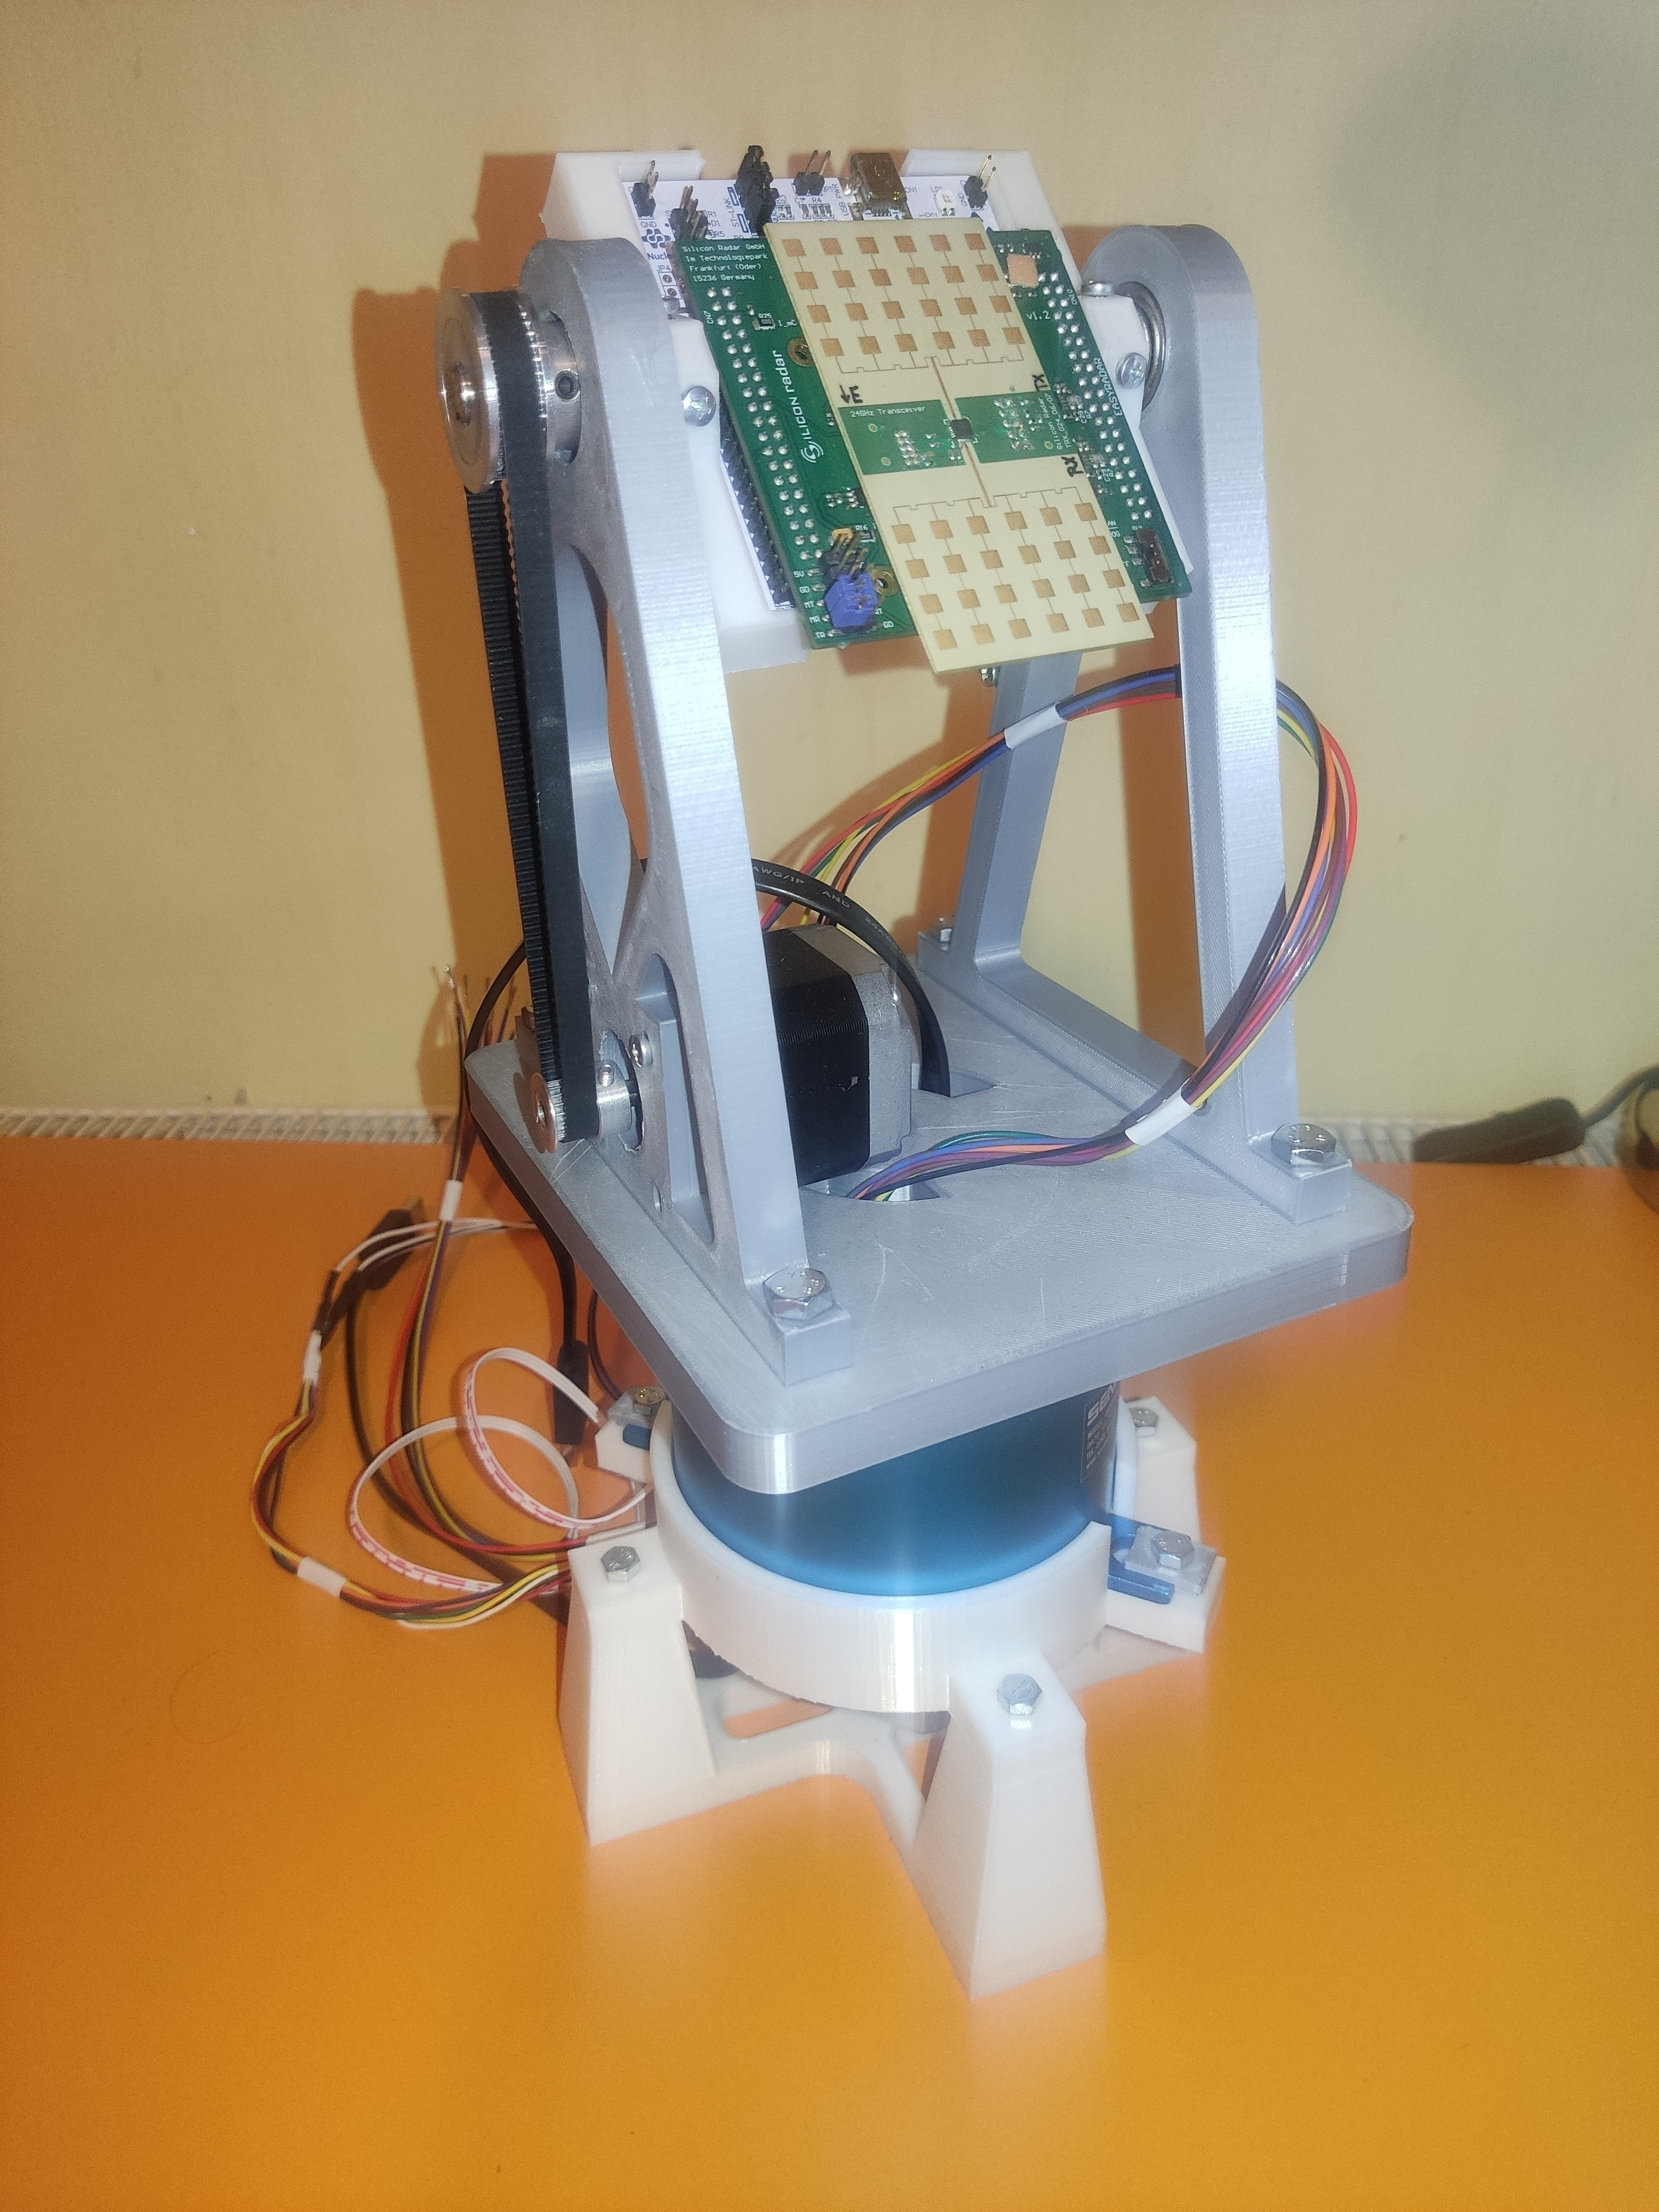
\includegraphics[width=0.75\textwidth]{../img/assembly_photo.jpg} % Replace with your image path
    \caption{Photo}
  \end{subfigure}
  \caption{Form of the final assembly}
  \label{fig:side_by_side}
\end{figure}

In stark departure from commercial solutions \cite{carl,standa} due to need to accommodate a large slipring first axis controls rotation and second one tilt.
This arrangement also leads to simpler calculation of speed vector, needed for radar processing, by reducing the interdependence of movements between each axis.


\subsection{Platform Electronics}

\boldred{
	TODO: total rewrite of this section, drop things about Hall effect, outlay a basic schema of what components are present and how are they connected.
	Keep it rather short if possible
}

% \red{
Electronic side of the project is rather simple given that only control of two stepper motors and having ability to home their position is needed.
The system is managed by an ESP32 microcontroller. Since the project does not demand advanced capabilities, a basic ESP32 model is sufficient.

Given the low load on stepper motors and the platform's inability to accumulate significant momentum, a simple stepper driver without feedback control is adequate.
For this purpose, the A4988 stepper driver was selected, due to its low cost, microstepping capabilities and basic current control \cite{a4988}.

To implement homing, two potential solutions were considered: Hall effect sensors and optical gates.
While Hall effect sensors offer the advantage of angle sensing, allowing correction of any positional drift during operation, they require precise alignment.
If the orthogonal Hall effect sensor is not perfectly placed in the axis of rotation, non simply calibration becomes a necessity \cite{hall}.

Thus for simplicity and ease of integration, optical gates were selected.
This decision eliminates the need for complex calibration while providing reliable functionality.
% }

\section{Platform Software Realization}

\boldblue{NOTE: Basic structure of this chapter is fine.}

To maximize efficiency in processing commands and ensure accurate stepper motor control, the program workflow is divided into three distinct layers, as illustrated by figure \ref{fig:code_diag}.

The commonly used two-component architecture—where one component handles communication/command parsing and the other manages execution—was deemed unsuitable for this use case.
Such an approach would complicate integration of programming interface and require just-in-time processing of commands, which could lead to performance issues.

In the chosen architecture, the degree of abstraction decreases with each successive layer, simplifying processing at each step.
This design allows the final layer to operate with maximum efficiency, where transition from one command to the next is primarily limited by the inertia of stepper motors and not by the software.

\begin{figure}[h!]
  \centering


  \begin{tikzpicture}[scale=0.9, node distance=1.5cm]

    % Layer headers
    \node (comm_layer) [layerheader] at (0, 0) {Communication Layer};
    \node (app_layer) [layerheader] at (6, 0) {Application Layer};
    \node (hal_layer) [layerheader] at (12, 0) {HAL Layer};

    % Communication Layer
    \node (comm_start) [startstop, below of=comm_layer, yshift=-0.3cm] {Start};
    \node (wait_serial) [process, below of=comm_start] {Wait for serial data};
    \node (parse_gcode) [process, below of=wait_serial] {Parse G-code};
    \node (parse_success) [decision, below of=parse_gcode, align=center, yshift=-1.3cm] {Parsing\\ Successful?};
    \node (store_command) [process, below of=parse_success, align=center, yshift=-1.8cm] {Store command\\ queue ? program};
    \node (send_response) [process, below of=store_command,yshift=-0.25cm] {Send response};

    % Arrows in Communication Layer
    \draw [arrow] (comm_start) -- (wait_serial);
    \draw [arrow] (wait_serial) -- (parse_gcode);
    \draw [arrow] (parse_gcode) -- (parse_success);
    \draw [arrow] (parse_success.east) -- ++(1, 0) |- (send_response.east) node[midway, left, yshift=+0.25cm] {No};
    \draw [arrow] (parse_success.south) -- ++(0, -0.5) -| (store_command.north) node[midway, right, yshift=+0.05cm] {Yes};
    \draw [arrow] (store_command) -- (send_response);
    \draw [arrow] (send_response.west) -- ++(-0.5, 0) |- (wait_serial.west);

    % Application Layer
    \node (app_start) [startstop, below of=app_layer, yshift=-0.3cm] {Start};
    \node (update_position) [process, below of=app_start] {Update position};
    \node (check_queues) [decision, below of=update_position, yshift=-1.3cm] {Queues full?};
    \node (load) [process, below of=check_queues, align=center, yshift=-1.5cm] {Load command \\ queue ? program};
    \node (process_command) [process, below of=load,yshift=-0.25cm] {Process command};
    \node (store_command) [process, align=center, below of=process_command] {Add command \\ to stepper queue};

    % Arrows in Application Layer
    \draw [arrow] (app_start) -- (update_position);
    \draw [arrow] (update_position) -- (check_queues);
    \draw [arrow] (check_queues.east) -- ++(1, 0) |- (update_position.east) node[midway, left, xshift=0.2cm, yshift=+0.25cm,xshift=0.2cm] {Yes};
    \draw [arrow] (check_queues.south) -- ++(0, -0.5) -| (load.north) node[midway, right, yshift=+0.1cm] {No};
    \draw [arrow] (load.south) -- ++(0, -0.5) -- (process_command.north);
    \draw [arrow] (process_command) -- (store_command);
    \draw [arrow] (store_command.west) -- ++(-0.5, 0) |- (update_position.west);


    \node (hal_start) [startstop, below of=hal_layer, yshift=-0.3cm] {Start};
    \node (wait_queue) [process, below of=hal_start] {Wait on queue};
    \node (execute_command) [process, below of=wait_queue] {Execute command};
    \node (wait_command) [process, below of=execute_command] {Wait on command};
    \node (update_info) [process, align=center, below of=wait_command] {Update last \\command};

    % Arrows in HAL Layer
    \draw [arrow] (hal_start) -- (wait_queue);
    \draw [arrow] (wait_queue) -- (execute_command);
    \draw [arrow] (execute_command) -- (wait_command);
    \draw [arrow] (wait_command) -- (update_info);
    \draw [arrow] (update_info.west) -- ++(-0.5, 0) |- (wait_queue.west);

  \end{tikzpicture}

  \caption[Programm diagram]{Programm diagram}
  \label{fig:code_diag}
\end{figure}

\subsection{Communication layer}

The communication layer manages incoming data over the serial line, with efficient handling facilitated with the aid of RTOS queues.
Upon receiving data the text string is parsed and either pushed to a queue or added to programm declaration, in case we are currently declaring program.

Immediately after parsing, a response is send to the user confirming whether the command was parsed correctly or not.
However, as the communication layer does not a can not check command within context of all previous commands, it is possible that command will be parsed correctly but its execution will fail in the application layer.


\subsection{Application layer}

The application layer performs two primary functions: tracking the current device position and scheduling commands to be sent to stepper motors.
Aside from current position the program also keeps track of the end position of the last scheduled command.
Thanks to this the application layer make necessary calculations to facilitate absolute positioning and enforce movement limits.

A key departure from standard G-code interpreters, like \cite{duet}, is how the platform handles single-axis move commands.
When a move command targets only one axis, the other axis remains free to read next command and begin its execution.
If this behavior is undesirable, the user must issue commands for both axes.
In relative positioning mode, a zero value results in no motion; in absolute positioning mode, the command must specify the current position to prevent movement.

This behavior is a necessary side effect of the spindle regime, which typically cannot be toggled on or off dynamically.
Another consequence is the requirement for separate positioning modes for each axis.
Continuous rotation prevents calculations of a move’s end position, making it impossible to make calculation for absolute positioning commands -- thus necessitating relative positioning.
However it would be rather restrictive to force user to relative positioning on second axis, therefore the independent positioning settings.




\subsection{HAL Layer}

\boldred{TODO: Drop primitive equation which is totaly unnecessary and was only included to comply with the original assigment}

The final layer manages stepper motor control and provides the application layer with essential data for position calculations.
In its loop, the program waits for the next command in the stepper queue.
Upon receiving a command, it sets up execution, waits for one or both steppers to complete their movement, and then proceeds to the next command.
Since limit and absolute positioning calculations are handled in the application layer whole routine remains highly efficient.

The main challenge lies in generating precise PWM signals (Used to control stepper motors drivers.) and stopping signal generation after a specific number of steps.
Using the equation:
%
\begin{equation}
  t_{\mathrm{delay}}(s) = \frac{60}{2\cdot N_{\mathrm{steps}} \cdot s},
  \label{eq:delay}
\end{equation}
%
where $s$ is speed in RPM, $N_{\mathrm{steps}}$ is the number of steps (Anywhere from 200 to 1600 depending on microstepping.), and $t_{\mathrm{delay}}$ is the time between steps, we calculate that even at 30 RPM, the delay between output changes is 5 ms per step.
With microstepping at a 2:1 ratio, this reduces to 2.5 ms -- faster than lowest sleep interval on ESP32 and without sleeping the RTOS watchdog will trigger.
Therefore, signal generation must leverage specialized microcontroller peripherals.

The ESP32 platform offers two options: Remote Controlled Transceiver (RMT) and Motor Control Pulse Width Modulation (MCPWM) combined with Pulse Counter (PCNT).
While RMT allows smooth PWM frequency adjustments, it has several drawbacks.
Such as the fact that generating a specific number of pulses is supported only on newer ESP32 models \cite{gitRMT}, synchronization is restricted to its proprietary API, and there is no straightforward way to track progress during a move \cite{espRMT}.

For these reasons, MCPWM and PCNT were chosen.
MCPWM handles pulse generation, while PCNT counts steps, enabling easy synchronization, continuous rotation, and a robust API for step tracking \cite{espPCNT}.
The only limitation is the PCNT’s 15-bit counter, which caps the maximum steps per move at 32.767.


\subsubsection{Performance of the HAL Layer}

\boldred{TODO: Including Measurement is not a bad idea however the table is totaly redundant and doesn't provide much.}

Table \ref{tab:performancepwm} illustrates the stability of PWM generation by the MCPWM module at various speeds.
Measurements were conducted using a Saleae Logic Pro 16 logic analyzer, with no microstepping enabled.

The results show that frequency deviation is minimal, though the generated speed is consistently marginally faster than the target, and  the error increases slightly with higher speeds.
Nevertheless, when measuring time of 24,000 steps at 120 RPM, the relative error in time duration (or speed) was only $\epsilon = -0.004\%$, demonstrating excellent accuracy.


\begin{table}[h!]
  \centering
  \caption[Stability of PWM generation]{Stability of PWM generation}
  \begin{tabular}{| m{2cm} || m{2.5cm} | m{2.5cm} | m{2.5cm} | m{2.5cm} |}
    \hline
    RPM & $f_{\mathrm{desired}}$ (Hz) & $f_{\mathrm{low}}$ (Hz) & $f_{\mathrm{high}}$ (Hz) & $f_\mathrm{avg}$ (Hz) \\
    \hline
    10  & 33.334                      & 33.334                  & 33.334                   & 33.334                \\
    30  & 100                         & 100                     & 100.003                  & 100.002               \\
    60  & 200                         & 200                     & 200.01                   & 200.004               \\
    120 & 400                         & 400                     & 400.02                   & 400.007               \\
    \hline
  \end{tabular}
  \label{tab:performancepwm}
\end{table}

\begin{figure}[h!]
	\centering
	\includegraphics[width=0.7\textwidth]{../img/120rpm_to60_1.jpg}
	\includegraphics[width=0.7\textwidth]{../img/120rpm_to60_2.jpg}
	\caption[Moment of change between commands with 120RPM and 60RPM]{Moment of change between commands (120RPM $\Rightarrow$  60RPM)}
	\label{fig:switching}
\end{figure}

An attempt was made to also measure the delay  between switching commands, displayed in figure \ref{fig:switching}.
The results indicate that the delay between commands is imperceptible.
Similar outcomes were also observed for other command combinations.

This demonstrates the efficiency of the HAL layer in managing stepper motor control and transitioning seamlessly between commands.
As long as stepper queues are supplied with commands in advance, the platform can operate without noticeable interruptions.
Most importantly, the platform’s timely and predictable behavior ensures that mathematical corrections to the radar data can be applied accurately.


% vim.ft=tex
\chapter*{Conclusion}
\addcontentsline{toc}{chapter}{Conclusion}

Goal of this thesis was to realize a surveillance radar system based on FMCW technology.
This technology should enable accurate distance measurements of targets with a relatively low power consumption.
Instead of more conventional MIMO systems, a simpler solution was proposed with a single RX and TX antenna that relies on mechanical steering of the radar beam.

Using off-the-shelf components and 3D printed parts a custom rotary platform was designed and constructed.
All be it minor issues in regards to the belt tension on pitch axes in enables controlling of the radar position in both yaw and pitch directions.
Quality of life features such a automatic homing system or limits to the rotation were also implemented.
Whole system is controlled by an ESP32C6 microcontroller which interprets G-code like commands and drives the stepper motors.
Due to its similarities to other G-code base systems it should be readily adaptable to other systems.
In addition the platform was designed to support capabilities that aren't strictly necessary for the purpose of this thesis.

Capabilities of \sidar evaluation board were analyzed and were found to be suitable for the purpose of this thesis.
However not much room is left to improvement of the system as the board is limited by its low sampling rate and relatively slow microcontroller.
This limits the maximum detectable speed to tens of mm per second which effectively eliminates any possibility of tracking moving targets.
However it's ability to switch headers between 24~GHz and 122~GHz allows for a wide range of applications.

Control application for the system was developed in MATLAB.
This integrates both the rotary platform management and radar data processing.
Given rather generic design requirements of the application, larger degree of customization is allowed with simpler GUI menu.
The data processing pipeline is relatively standard reling on common techniques such as FFT, CFAR, DBSCAN and others.
Major downside is that configuration must be tailored to specific application and therefore the user must have a good understanding radar processing and some knowledge of the processing pipeline.
No predefined configurations for specific usecase are provided in the application.


FIX TODO

In addition whole processing is written in a way that if radar module was exchanged for a faster one capabilities could be much more extended without requring
keeping most of the codebase similar.
Aside from different function reading the data from the radar all code is relatively lightweight till the point position change is detected and multiple fft spectrums are being processed.

Thus radar with just increased chirp frequency would only lead to better speed recognition.
Especially if platform movement remained the same.
In case  of increase of platform rotation possible corrections would need to be done in the processing pipeline.

In case number of FFT points both in speed or range would be significantly larger that what has been tested (Maximal cube dimensions of around 500~MB were validated) different approach to cube update would be required.
First possibility would be leverages GPU acceleration to handle operations in the cube update.
Specifically the decaying of the cube would be possible for much larger dimensions.
In case of solely CPU based processing decay functions probably would be impractical for much larger cubes and the cube would need to be split into smaller chunks where only few ones would be loaded into RAM at one time -- depending on the current position of the platform and direction of travel.





\include{bibliography}

\listoffigures

\listoftables

\clearpage
\openright
\end{document}
